\documentclass{beamer}

\usepackage{préambule}

\begin{document}

\newcommand{\computeF}[1]{0.05*(#1+3)*(#1+1)*(#1-4)}
\newcommand{\Graphique}[1][]{
	\begin{tikzpicture}[#1]
		\draw[\myArrow] (-5.5,0) -- (5.5,0);
		\draw[\myArrow] (0,-4) -- (0,4);

		\draw[orange,thick,domain=-5:5,variable=\x] plot({\x},{0.05*(\x+3)*(\x+1)*(\x-4)}) node[above] {$𝒞_f$};

		\draw[dashed] (-5,0) node[above] {$-5$} -- (-5,-3.6) -- (0,-3.6) node[right] {$-3,6$};
		\draw[dashed] (-2,0) node[below] {$-2$} -- (-2,0.3) -- (0,0.3) node[right] {$0,3$};
		\draw[dashed] (2,0) node[above] {$2$} -- (2,-1.5) -- (0,-1.5) node[left] {$-1,5$};
		\draw[dashed] (5,0) node[below] {$5$} -- (5,2.4) -- (0,2.4) node[left] {$2,4$};
	\end{tikzpicture}
}

\begin{frame}
	Donner le tableau de signes de la fonction suivante :
	\begin{center}
		\begin{tikzpicture}[scale=0.9]
			\draw[\myArrow] (-5.5,0) -- (5.5,0);
			\draw[\myArrow] (0,-4) -- (0,4);

			\draw[orange,thick,domain=-5:5,variable=\x] plot({\x},{0.05*(\x+3)*(\x+1)*(\x-4)}) node[above] {$𝒞_f$};

			\draw[dashed] (-5,0) -- ++(0,0.2) node[above] {$-5$} -- (-5,-3.6);
			\draw (-3,0) -- ++(0,-0.2) node[below] {$-3$};
			\draw (-1,0) -- ++(0,-0.2) node[below] {$-1$};
			\draw (4,0) -- ++(0,-0.2) node[below] {$4$};
			\draw[dashed] (5,0) -- ++(0,-0.2) node[below] {$5$} -- (5,2.4);
		\end{tikzpicture}
	\end{center}
\end{frame}

\begin{frame}
	\begin{center}
		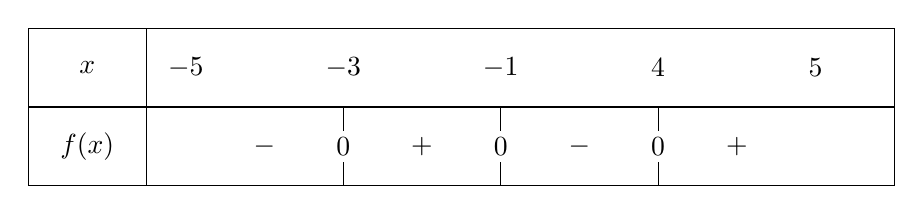
\begin{tikzpicture}
			\draw (0,0) -- ++(11,0) -- ++(0,-2) -- ++(-11,0) -- cycle;
			\draw (0,-1) -- ++(11,0);
			\draw (1.5,0) -- ++(0,-2);

			\node at (0.75,-0.5) {$x$};
			\node at (2,-0.5) {$-5$};
			\node at (4,-0.5) {$-3$};
			\node at (6,-0.5) {$-1$};
			\node at (8,-0.5) {$4$};
			\node at (10,-0.5) {$5$};

			\node at (0.75,-1.5) {$f(x)$};
			\node at (3,-1.5) {$-$};
			\node at (4,-1.5) {$0$};
			\node at (5,-1.5) {$+$};
			\node at (6,-1.5) {$0$};
			\node at (7,-1.5) {$-$};
			\node at (8,-1.5) {$0$};
			\node at (9,-1.5) {$+$};
			\draw (4,-1) -- ++(0,-0.3) ++ (0,-0.4) -- ++(0,-0.3);
			\draw (6,-1) -- ++(0,-0.3) ++ (0,-0.4) -- ++(0,-0.3);
			\draw (8,-1) -- ++(0,-0.3) ++ (0,-0.4) -- ++(0,-0.3);
		\end{tikzpicture}
	\end{center}
\end{frame}

\begin{frame}
	Donner le tableau de variations de la fonction suivante :
	\begin{center}
		\Graphique[scale=0.9]
	\end{center}
\end{frame}

\begin{frame}
	\begin{center}
		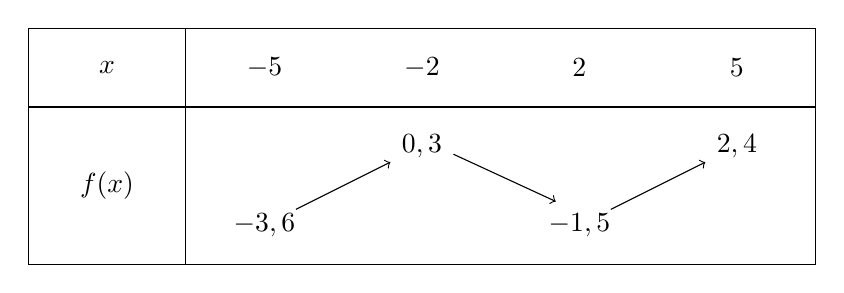
\begin{tikzpicture}
			\draw (0,0) -- ++(10,0) -- ++(0,-3) -- ++(-10,0) -- cycle;
			\draw (0,-1) -- ++(10,0);
			\draw (2,0) -- ++(0,-3);

			\node at (1,-0.5) {$x$};
			\node at (3,-0.5) {$-5$};
			\node at (5,-0.5) {$-2$};
			\node at (7,-0.5) {$2$};
			\node at (9,-0.5) {$5$};

			\node at (1,-2) {$f(x)$};
			\node at (3,-2.5) {$-3,6$};
			\node at (5,-1.5) {$0,3$};
			\node at (7,-2.5) {$-1,5$};
			\node at (9,-1.5) {$2,4$};

			\draw[->] (3.4,-2.3) -- ++(1.2,0.6);
			\draw[->] (5.4,-1.6) -- ++(1.3,-0.6);
			\draw[->] (7.4,-2.3) -- ++(1.2,0.6);
		\end{tikzpicture}
	\end{center}
\end{frame}

\begin{frame}
	\begin{center}
		\Graphique[scale=0.7]
	\end{center}

	Calculer :
	\begin{itemize}
		\item Le taux de variation de $f$ entre $-5$ et $-2$ : \correction{$1,3$}\vspace{0.5em}
		\item Le taux de variation de $f$ entre $-2$ et $2$ : \correction{$-0,36$}\vspace{0.5em}
		\item Le taux de variation de $f$ entre $2$ et $5$ : \correction{$1,3$}
	\end{itemize}
\end{frame}

\begin{frame}
	\begin{itemize}
		\item Le taux de variation de $f$ entre $-5$ et $-2$ est

		      $$ \dfrac{f(-2) - f(-5)}{-2 - (-5)} = \dfrac{0,3 - (-3,6)}{-2 - (-5)} = 1,3 $$
		\item Le taux de variation de $f$ entre $-2$ et $3$ est

		      $$ \dfrac{f(2) - f(-2)}{2 - (-2)} = \dfrac{-1,5 - 0,3}{2 - (-2)} = -0,45 $$
		\item Le taux de variation de $f$ entre $2$ et $5$ est

		      $$ \dfrac{f(5) - f(2)}{5 - 2} = \dfrac{2,4 - (-1,5)}{5 - 2} = 1,3 $$
	\end{itemize}
\end{frame}

\end{document}